\subsection{实验}
\label{sec:task3-experiments}

\subsubsection{数据预处理与划分}
\label{sec:exp:preprocessing}
实验读取 GBK 编码的气象数据，共有 $26{,}200$ 条记录、$21$ 个数值变量以及一列日期。预测目标为 CO$_2$ 浓度，单位为 ppm。当前程序先按 \texttt{date} 字符串排序，再将所有不大于 $-9998$ 的数值设为缺失，包括传感器占位值 $-9999$。原始数据共有 $45$ 处此类异常值，其中目标列占 $34$ 处。

缺失值在完整数据表上按当前行位置进行双向线性插值。对于有效观测位置 $a<t<b$，第 $j$ 个变量的填充值为
\begin{equation}
    x_{t,j}=x_{a,j}+\frac{t-a}{b-a}(x_{b,j}-x_{a,j}).
    \label{eq:interpolation}
\end{equation}
序列边缘的缺失值按双向补全规则处理，插值后数值列无缺失值。

清洗后以长度 $L=12$、步长为 $1$ 的滑动窗口构造单步预测样本，得到 $26{,}188$ 个 $12\times21$ 输入窗口。按处理后的样本索引连续划分训练、验证与测试集，样本数分别为 $17{,}809$、$3{,}142$ 和 $5{,}237$。测试集取全部样本的最后 $20\%$，验证集取剩余样本的最后 $15\%$。图~\ref{fig:target-distribution} 展示的是训练集、验证集和测试集的 CO$_2$ 浓度标签分布。

输入标准化器仅在训练窗口上拟合。第 $j$ 个特征的均值与总体方差由全部训练窗口中的观测位置计算：
\begin{align}
    \mu_j&=\frac{1}{M_{\mathrm{tr}}L}
    \sum_{i\in\mathcal{I}_{\mathrm{tr}}}\sum_{\tau=1}^{L}
    X_{i,\tau,j},
    \label{eq:mean}\\
    s_j^2&=\frac{1}{M_{\mathrm{tr}}L}
    \sum_{i\in\mathcal{I}_{\mathrm{tr}}}\sum_{\tau=1}^{L}
    (X_{i,\tau,j}-\mu_j)^2.
    \label{eq:variance}
\end{align}
训练、验证和测试集共用这组统计量，按式~\eqref{eq:standardization} 变换；目标值使用训练输入中 CO$_2$ 特征对应的均值和标准差缩放。

\begin{figure*}[!t]
  \centering
  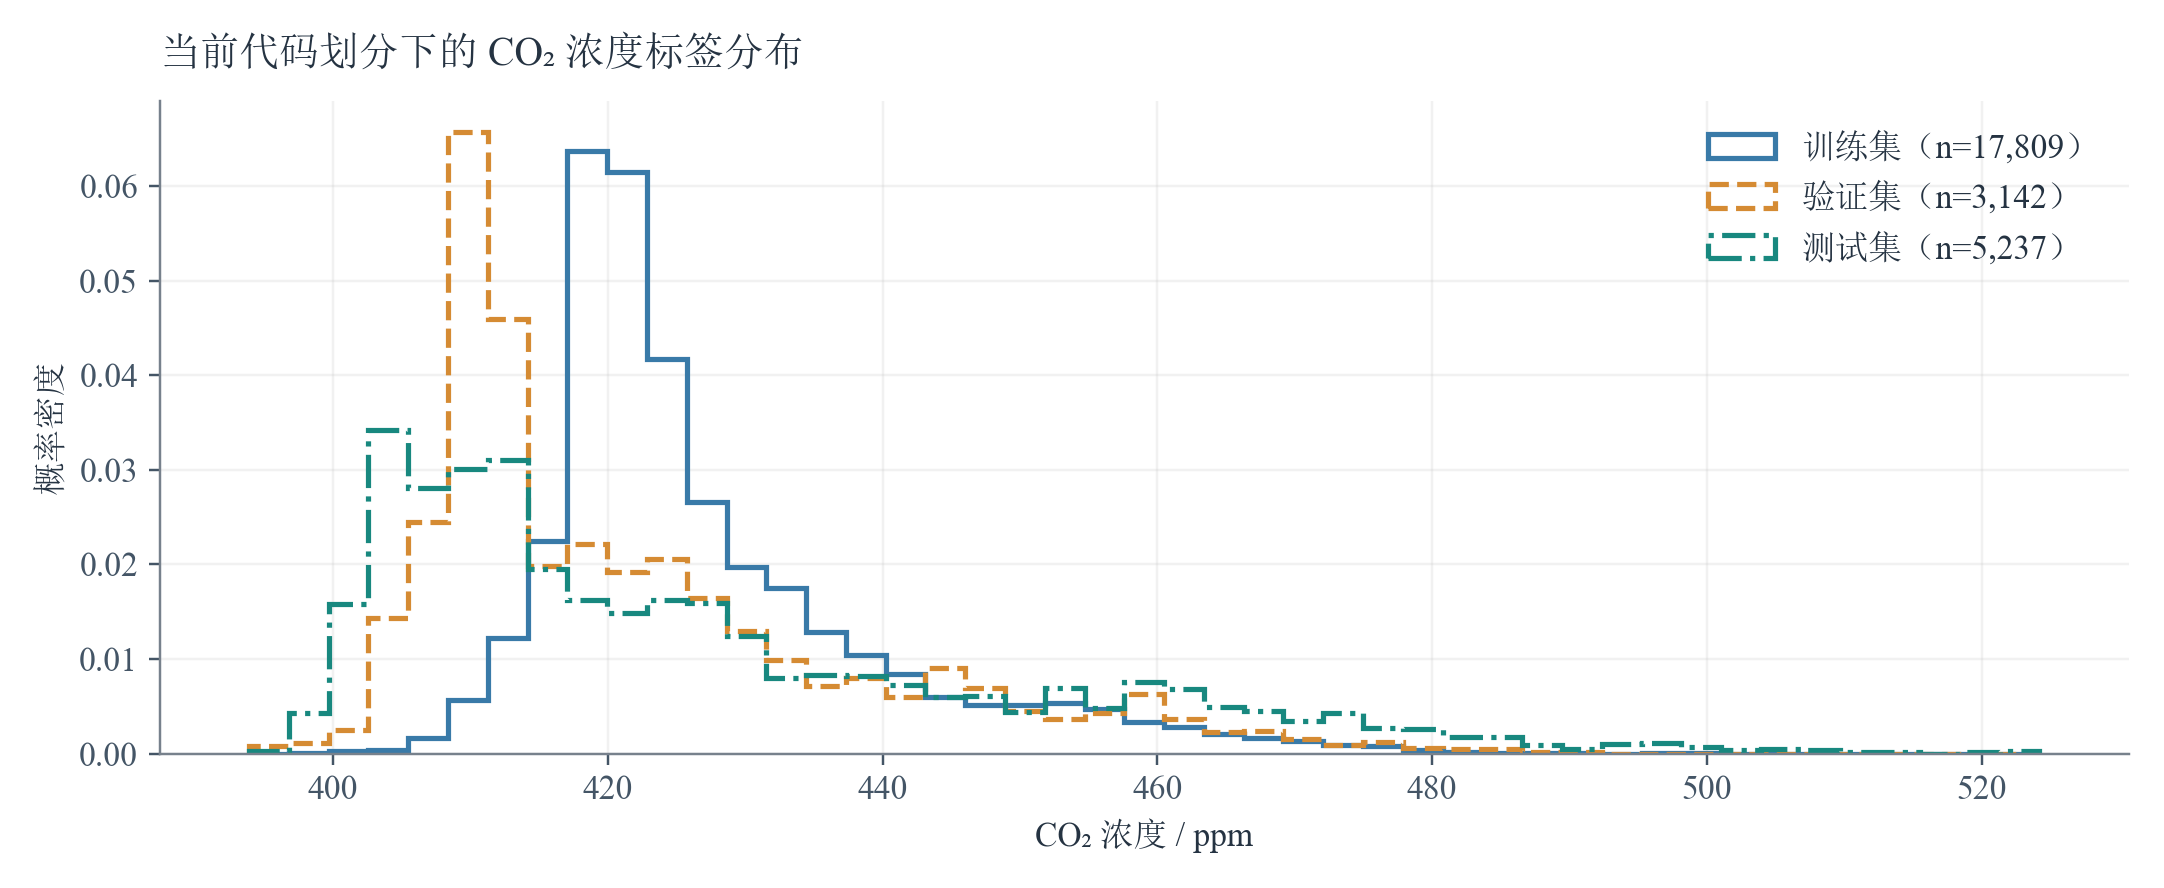
\includegraphics[width=0.88\textwidth]{figures/split_target_distribution.png}
  \Description{训练、验证和测试集的二氧化碳浓度分布直方图。}
  \caption{当前代码划分下的 CO$_2$ 浓度标签分布}
  \label{fig:target-distribution}
  \par\medskip
  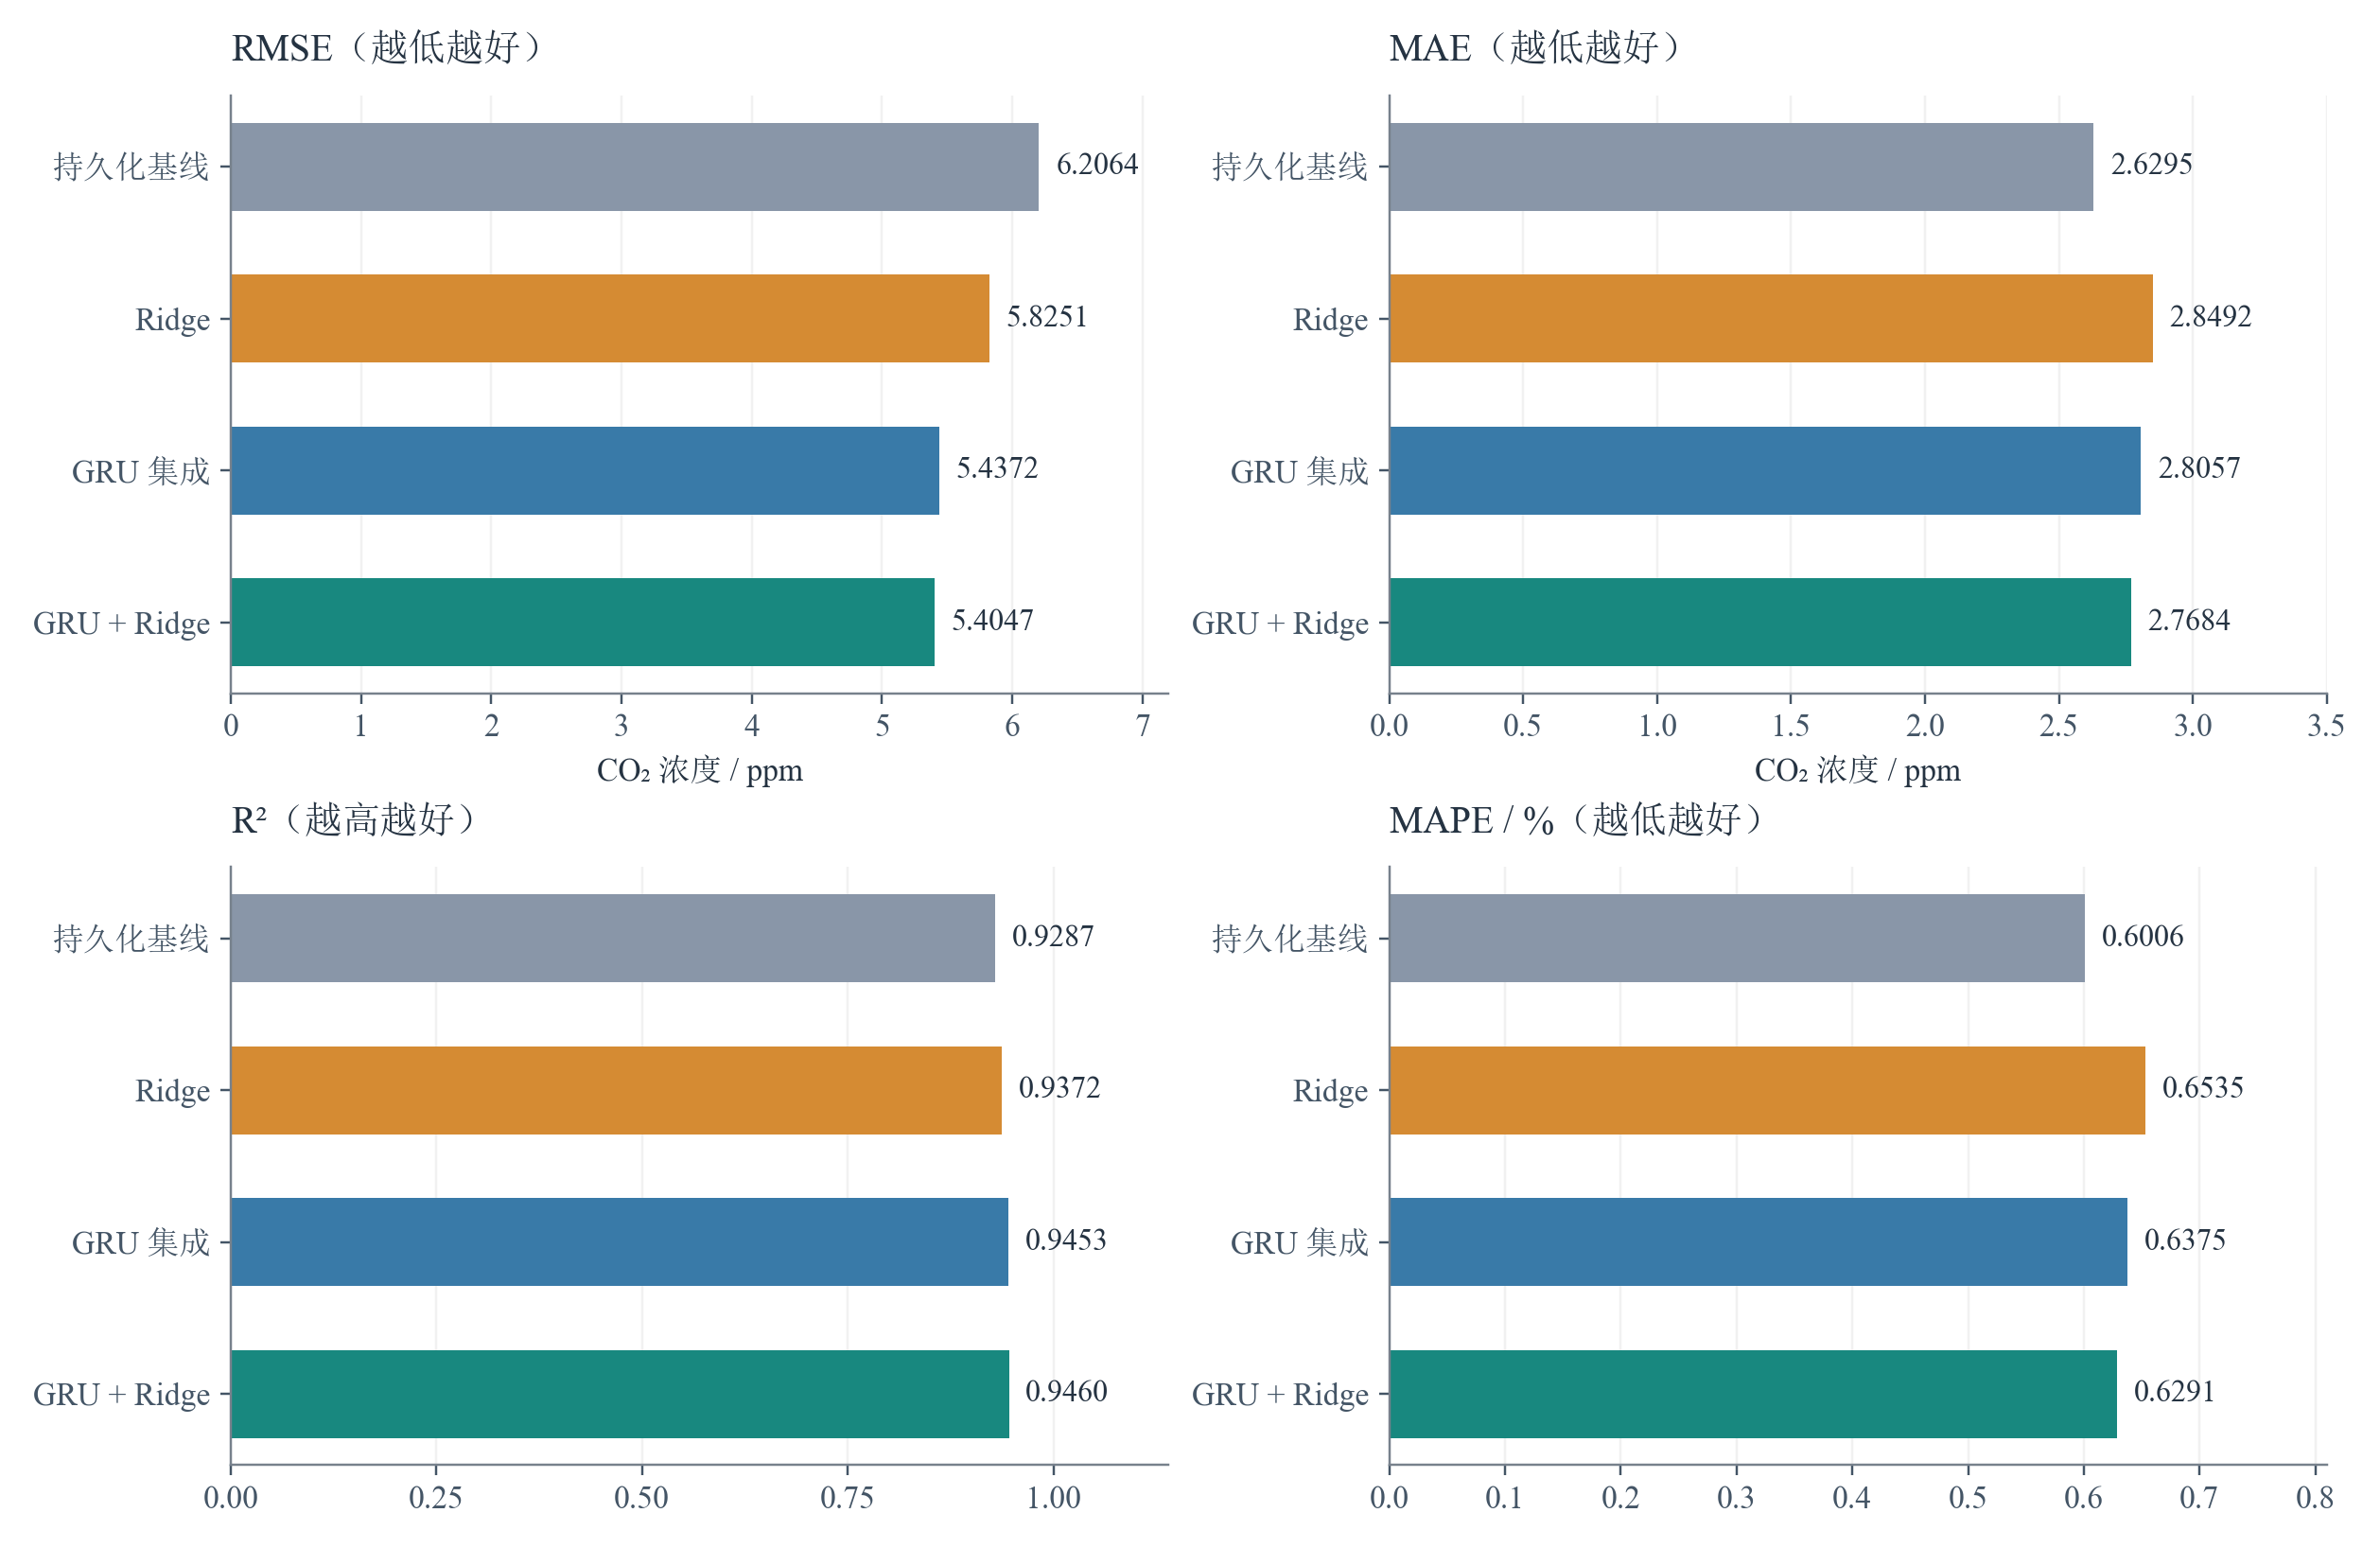
\includegraphics[width=0.88\textwidth]{figures/metrics_comparison.png}
  \Description{四组方法的 RMSE、MAE、决定系数与 MAPE 测试指标条形图。}
  \caption{当前模型与三个比较项的测试指标}
  \label{fig:metric-comparison}
\end{figure*}

\subsubsection{实验配置与训练细节}
\label{sec:exp:training}
GRU 分支使用两层单向循环网络，隐藏维度为 $H=128$，回归头的隐藏维度为 $d=64$，采用 $128\rightarrow64\rightarrow1$ 的全连接结构。单个预测器的参数集合 $\theta_k$ 包含两层 GRU 和回归头，共有 165,377 个可训练参数。集成成员数为 $K=5$，五个预测器合计包含 826,885 个神经网络参数。层间及回归头的 Dropout 比例均为 $p=0.2$。训练时，$\mathcal{D}_p$ 随机将部分分量置零，并将保留分量乘以 $1/(1-p)$；验证与测试时关闭 Dropout，该算子为恒等映射。

五个成员分别以种子 $0$ 至 $4$ 训练，批次大小为 $256$，最多训练 $200$ 轮，以式~\eqref{eq:gru_loss} 为损失函数。优化器为 Adam\citep{kingma2015adam}，初始学习率为 $5\times10^{-4}$，动量参数为 $\beta_1=0.9$、$\beta_2=0.999$，$\epsilon=10^{-8}$，权重衰减为零。每轮打乱训练窗口的送入顺序而保持窗口内部排列不变，反向传播后将全局梯度范数裁剪至不超过 $1$。训练损失在标准化标签上计算；对同一组预测，还原为 ppm 后的 MSE 等于 $s_y^2\mathcal{L}_{\mathrm{G}}$，因此两种量纲下的 MSE 排序相同。

每轮结束后在完整验证集上计算 MSE。学习率调度器的容忍计数为 $8$、衰减因子为 $0.5$、最低学习率为 $10^{-6}$。验证损失连续 $25$ 轮未超过 $10^{-6}$ 的改善阈值时触发早停，训练结束后恢复验证损失最优的参数。训练种子在模型构建后设置，作用于后续训练过程。

岭回归独立于 GRU 拟合，包含 $LF$ 个系数和一个截距，式~\eqref{eq:ridge_loss} 的正则化参数取 $\alpha=1$。

GRU 集成按式~\eqref{eq:ensemble} 对五个成员的预测取均值，作为集成分支的输出。两条分支完成训练后，固定各自的参数，在候选集合 $\mathcal{W}=\{0,0.05,\ldots,0.95,1\}$ 中搜索融合权重。记验证样本索引集为 $\mathcal{I}_{\mathrm{va}}$，通过最小化验证集 MSE 选择全局组合系数：
\begin{equation}
    w^*=\underset{w\in\mathcal{W}}{\arg\min}\;
    \frac{1}{|\mathcal{I}_{\mathrm{va}}|}
    \sum_{i\in\mathcal{I}_{\mathrm{va}}}
    \bigl(w g_i+(1-w)r_i-\widetilde{y}_i\bigr)^2.
    \label{eq:fusion_selection}
\end{equation}
候选集合包含 21 个权重，保存的最优 GRU 权重为 $0.95$。GRU 参数、岭回归系数和融合权重由三个独立阶段确定，融合系数不参与神经网络的梯度更新，测试标签不参与权重搜索。测试阶段固定已选择的模型参数、标准化统计量与融合权重，不使用验证集重新拟合分支。对照项包括持久化预测、独立 Ridge 和五个 GRU 的预测均值；这些比较项用于解释当前融合模型的效果。

\subsubsection{评价指标}
所有指标均在反标准化后的测试集预测上计算。记测试样本数为 $n=5{,}237$，真实值为 $y_i$，预测值为 $\widehat y_i$，测试集真实值均值为 $\bar y=n^{-1}\sum_{i=1}^{n}y_i$。采用均方根误差（RMSE）、平均绝对误差（MAE）、决定系数（$R^2$）和平均绝对百分比误差（MAPE）：
\begin{align}
\mathrm{RMSE}
  &=\sqrt{\frac{1}{n}\sum_{i=1}^{n}(y_i-\widehat y_i)^2},\\
\mathrm{MAE}
  &=\frac{1}{n}\sum_{i=1}^{n}|y_i-\widehat y_i|,\\
R^2
  &=1-\frac{\sum_{i=1}^{n}(y_i-\widehat y_i)^2}
            {\sum_{i=1}^{n}(y_i-\bar y)^2},\\
\mathrm{MAPE}(\%)
  &=\frac{100}{n}\sum_{i=1}^{n}
    \left|\frac{y_i-\widehat y_i}{y_i}\right|.
\end{align}
RMSE 和 MAE 的单位为 ppm，数值越低越好；$R^2$ 越高越好。

\subsubsection{实验结果与分析}
表~\ref{tab:task3-results} 展示了 GRU--Ridge 融合模型与各对照方法在测试集上的预测性能。融合模型在 RMSE 和 $R^2$ 上取得最优值，分别为 $5.4047$ ppm 和 $0.9460$。相较独立 GRU 集成，融合后的 RMSE 从 $5.4372$ ppm 降至 $5.4047$ ppm，下降约 $0.60\%$；MAE 从 $2.8057$ ppm 降至 $2.7684$ ppm，下降约 $1.33\%$。

\begin{table*}[t]
  \caption{当前实现的测试集结果。粗体表示每列最优值。}
  \label{tab:task3-results}
  \centering
  \begin{tabular}{lcccc}
    \toprule
    方法 & RMSE $\downarrow$ & MAE $\downarrow$ & $R^2$ $\uparrow$ & MAPE (\%) $\downarrow$\\
    \midrule
    持久化预测 & 6.2064 & \textbf{2.6295} & 0.9287 & \textbf{0.6006}\\
    Ridge & 5.8251 & 2.8492 & 0.9372 & 0.6535\\
    GRU 集成 & 5.4372 & 2.8057 & 0.9453 & 0.6375\\
    GRU + Ridge（当前模型） & \textbf{5.4047} & 2.7684 & \textbf{0.9460} & 0.6291\\
    \bottomrule
  \end{tabular}
\end{table*}

图~\ref{fig:metric-comparison} 展示的是持久化预测、Ridge、GRU 集成和融合模型在 RMSE、MAE、$R^2$ 与 MAPE 四项指标上的测试结果。以持久化预测为参照，融合模型的 RMSE 与 MAE 相对变化分别为 $-12.92\%$ 和 $+5.28\%$。

\begin{figure}[!htbp]
  \noindent 图~\ref{fig:scatter} 展示的是测试集 CO$_2$ 浓度预测值与真实值的散点分布，散点总体沿 $\widehat y=y$ 分布。
  \par\medskip
  \centering
  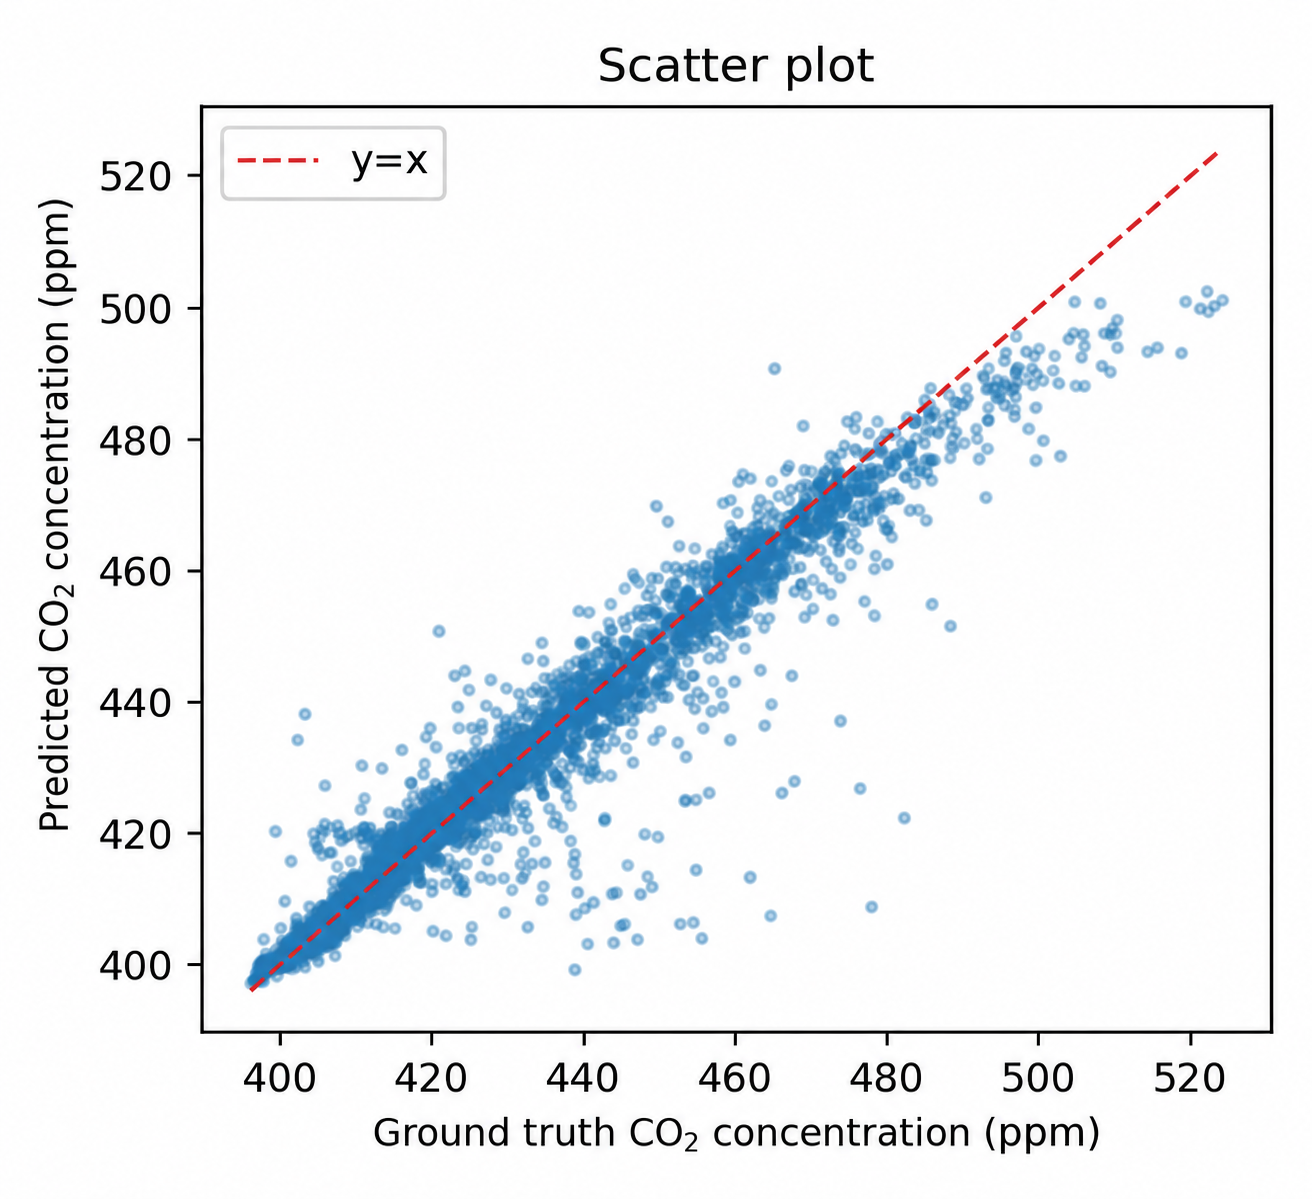
\includegraphics[width=\linewidth]{figures/scatter.png}
  \Description{融合模型预测与真实二氧化碳浓度的散点图及对角参考线。}
  \caption{测试集 CO$_2$ 浓度预测值与真实值的散点图}
  \label{fig:scatter}
\end{figure}

\FloatBarrier
